\documentclass{article}

\usepackage[margin=2cm]{geometry}

\usepackage{amsmath}
\usepackage{amsfonts}
%\usepackage{braket}
\usepackage{tabularx}
\usepackage{amsthm}
\usepackage[braket, qm]{qcircuit}
\usepackage[bookmarks = true, pdfpagemode = None, pdfstartview = FitH, colorlinks = true, urlcolor = blue]{hyperref}
\usepackage{listings}
\usepackage{caption}
\usepackage{subcaption}
\usepackage{graphicx}
\usepackage{algorithm}
\usepackage[noend]{algpseudocode}
\makeatletter
% Reinsert missing \algbackskip
\def\algbackskip{\hskip-\ALG@thistlm}
\makeatother
\renewcommand{\arraystretch}{1.5}

\theoremstyle{definition}
\newtheorem{definition}{Definition}[section]

\theoremstyle{problem}
\newtheorem{problem}{Problem}[section]

\theoremstyle{lemma}
\newtheorem{lemma}{Lemma}[section]

\title{PhD Project Report\\Optimal Designs for Fault-Tolerant Quantum Computers}
\author{Author: Luke Heyfron\\Supervisor: Dr. Earl T. Campbell}
\date{June 2017}

\begin{document}
	\captionsetup{width=0.8\linewidth}
	\maketitle
	
	\section{Introduction}
	Certain high threshold quantum error correction codes such as the toric code have transversal implementations of quantum logic gates that generate the logical Clifford group.
	However, the Clifford group in isolation is insufficient for universal quantum computation: one quantum gate outside the Clifford group must be included in the gate set.
	This is often chosen to be the T gate, which unfortunately does not have a transversal implementation on the toric code.
	A standard way to apply a T gate fault-tolerantly to a logically encoded qubit is to prepare a high-fidelity ancillary T-type magic state using magic state distillation protocols, then apply a teleportation gadget between the ancilla and the target qubit. This method involves many more elementary gates than the transversal Clifford gates, which motivates the cost model for logical quantum gates where the Clifford gates are ``free" and T gates are ``expensive". Consequentially, it is of interest to find ways to reduce the number of T gates used in implementations of quantum circuits.
	
	Previous work in this area.
	
	In this report an algorithm is presented for reducing the T count for $n$-qubit quantum circuits composed of CNOT and T gates. It is shown how it is possible to generalize this algorithm for the universal gate set $\{H, CNOT, T\}$. The rest of the paper is structured as follows: section \ref{s2_Theory} we define the terminology and notation conventions used for the rest of the paper; section \ref{s3_Problem} we define the problem in terms of quantum circuits and operators as well as in terms of a special kind of matrix representation, which facilitates the description of our solution. In section \ref{s4_Solution} we describe the algorithm presented in this paper for reducing the T count; in section \ref{s5_Results} we present the results of simulations of this algorithm compared to previous algorithms for both randomized circuits over CNOT and T as well as practical circuits of a universal gate set. Finally, we consolidate our results and discuss future work in section \ref{s6_Discussion}.
	
	\section{Theory and Terminology}
	\label{s2_Theory}
		\subsection{Quantum Theory}
		We define the set of $n$-qubit computational basis states to be $\{\ket{x}\}$ for all $x \in \{0,1\}^n$, the set of binary tuples of length $n$.
		
		The single qubit Pauli operators are defined in the computational basis as follows,
		\begin{equation}
		\label{e1_Paulis}
		\begin{matrix}
		\sigma_0 = \begin{pmatrix}1 & 0 \\ 0 & 1\end{pmatrix} & \sigma_x = \begin{pmatrix}0 & 1 \\ 1 & 0\end{pmatrix} \\
		& \\
		\sigma_y = \begin{pmatrix}0 & -i \\ i & 0\end{pmatrix} & \sigma_z = \begin{pmatrix}1 & 0 \\ 0 & -1\end{pmatrix}.
		\end{matrix}
		\end{equation}
		The $n$-qubit Pauli group $\mathcal{P}^n$ is defined as the $n$-fold tensor product of single qubit Pauli operators, along with multiplicative factors of $\pm1$ and $\pm i$ i.e. $\mathcal{P}^n = \{\left(-1\right)^a i^b \sigma_c \mid a,b \in \{0,1\}, c \in\{0,x,y,z\}\}^n$.
		
		The operators CNOT, H and T are given by
		\begin{equation}
		\label{e2_CNOT}
		\text{CNOT} = \begin{pmatrix}
		1 & 0 & 0 & 0 \\
		0 & 1 & 0 & 0 \\
		0 & 0 & 0 & 1 \\
		0 & 0 & 1 & 0
		\end{pmatrix},
		\end{equation}
		\begin{equation}
		\label{e3_H}
		H = \frac{1}{\sqrt{2}}\begin{pmatrix}
		1 & 1 \\
		1 & -1
		\end{pmatrix},
		\end{equation}
		\begin{equation}
		\label{e4_T}
		T = \begin{pmatrix}
		1 & 0 \\
		0 & \omega
		\end{pmatrix},
		\end{equation}
		where we define $\omega=e^{i\frac{\pi}{4}}$. A single qubit operator $G$ applied to the $i^\text{th}$ qubit of an $n$-qubit system is expressed as $G^{\left(i\right)}$. A controlled-$G$ operator where $G$ is a single qubit target operator is expressed as $\text{control-}G^{\left(t,c\right)}$ where the $t^\text{th}$ and $c^\text{th}$ qubits are the target and control qubit, respectively.
		
		The $n$-qubit Clifford group $\mathcal{C}^n$ is defined as the set of operators that maps $\mathcal{P}^n$ to itself under conjugation, $\mathcal{C}^n = \{U \mid UPU^\dagger = P^\prime, P, P^\prime \in \mathcal{P}^n\}$.
		
		The $k^{\text{th}}$ level of the Clifford hierarchy on $n$-qubits, $\mathcal{C}_k^n$, is defined inductively,
		\begin{equation}
		\mathcal{C}_k^n = \{U \mid UPU^\dagger = Q, P \in \mathcal{P}^n, Q \in \mathcal{C}_{k-1}^n\},
		\end{equation}
		with $\mathcal{C}_1^n = \mathcal{P}^n$.
		
		We define $\mathcal{D}_k^n \subseteq \mathcal{C}_k^n$ as the set of diagonal elements of the $k^{\text{th}}$ level of the Clifford hierarchy.
		
		\subsection{Classical Coding Theory}
		
		\subsection{Reed-Muller Codes}
		
		\subsection{Notes}
		NOTE: use mathbf for all matrices and vectors
	
	\section{The Gate Synthesis Problem}
	NOTES from Earl's paper:
		- magic states model formalized by Bravyi and Kitaev
		- Clifford operations are natively protected against noise in many error correcting codes including 2D topological codes such surface codes and 2D color codes.
		- Clifford operations: preparation of |0> states, measurement of Pauli group operators, Clifford group operators (normalizer of Pauli group), classical feed forward, access to classical random number generator.
		- Non-Clifford operations aren't natively protected so are costly.
		- Magic state distillation required (multiple layers) each of which involves many Clifford operations. Therefore, cost of non-clifford operations is significantly more than clifford operations
		- We measure resources by counting the number of logical T gates used in a circuit.
		- Using Campbell and Howard's synthillation protocol, the circuits can be implemented fault tolerantly with low overhead.
	
	An $n$-qubit quantum circuit $C$ of length $k$ is a time-ordered set of operators taken from an elementary gate set $G$ on $n$ qubits. For instance, if $C$ is such a quantum circuit, then $C = \{C_1,C_2,...,C_k\}$ where $C_t\in G^n$ is the operator applied at the $t^\text{th}$ time step.
	
	If $C$ is a quantum circuit, then $C$ is said to implement the unitary $U_C$, which is given by
	\begin{equation}
	U_C = \prod_{t = k}^1 C_t.
	\end{equation}
	Two circuits are said to be equivalent if they implement the same unitary. I.e. $C \equiv_U C^\prime$ if $U_C = U_{C^\prime}$. We define $E(g)$ to be the cost function of applying a particular gate $g\in G$ to a logical qubit. The total cost of a circuit is therefore,
	\begin{equation}
	\label{e_Cost}
	E(C) = \sum_{t=1}^k E(C_t).
	\end{equation}
	
	Given some initial circuit $C$, the gate synthesis problem is to find some circuit $C^\prime$ such that $\text{min}\{E(C^\prime) \mid U_{C^\prime} = U_C\}$.
	
	According to our cost model for quantum gates, $E(\text{Clifford}) = 0$ and $E(T)=1$. The total cost function for a circuit $C$ is therefore,
	\begin{equation}
	E(C) = \sum_{t=1}^k E(C_t) = \tau(C),
	\end{equation}
	where we define $\tau(C)$ to be the number of T gates in circuit $C$, which means the gate synthesis problem is equivalent to minimizing the number of T gates. We define the T count of a unitary $U$ as $\tau(U) = \text{min}\{\tau(C) \mid U = U_C\}$.
	
	\label{s3_Problem}
		\subsection{Circuits Composed of CNOT and T Gates}
	Any unitary $U$ generated by the CNOT and T gate can be decomposed as,
	\begin{equation}
	U = VW,
	\end{equation}
	where $V$ is a member of the Clifford group with $\tau(V)=0$ and $W \in \mathcal{D}_3^n$. It follows that $\tau(W) = \tau(U)$. Due to $V$ not contributing to the T count of $U$, we will assume that $U$ is already diagonal to simplify the analysis.
	
	The action of a unitary $U \in \mathcal{D}_3^n$ on a computational basis state can be written as follows,
	\begin{equation}
	U\ket{x} = \omega^{f_U(x)}\ket{x},
	\end{equation}
	where $f_U(x)$ is known as the \emph{phase function} for $U$. The phase function can be determined by tracking the state of each qubit through the circuit, updating appropriately after each CNOT gate, and adding a term after each T gate. This results in the general form for a phase function,
	\begin{equation}
	f_U(x) = \sum_{y\in\{0,1\}^n\backslash 0} \mathbf{a}_y \bigoplus_{i=1}^n x_i^{y_i}\mod 8,
	\end{equation}
	where $\mathbf{a}\in \mathbb{Z}_8^{2^n}$ is called an \emph{implementation vector}. Modulo 8 arithmetic is due to $\omega$ being the eight root of unity. This decomposition of the phase function is known as the \emph{phase polynomial} decomposition. Once an implementation vector for $U$ is found, it is possible to construct a circuit $C$ that implements $U$ using $\tau(C) = |\mathbf{a} \mod 2|$ T gates. There exist multiple implementation vectors that give rise to the same phase functions. This is due to the existence of non-trivial implementation vectors that implement the all-zero phase function.
	
	\theoremstyle{definition}
	\begin{definition}{Gate Synthesis Matrix.}
		Let $\mathbf{a}$ be an implementation vector for a phase function $f(x)$. A gate synthesis matrix is an $n\times m$ matrix, $A$, whose elements $A_{i,j} \in GF(2)$, where for each $y$ satisfying $(\mathbf{a}_{y} \mod 2)=1$, there is one column in $A$ such that $A_{i,j}=y_i$ for some $j \in \left[1,m\right]$.
	\end{definition}

	Note from the definition of a gate synthesis matrix, $m = |\mathbf{a} \mod 2|$, and that any two gate synthesis matrices that differ only by column permutations should be considered equivalent.
	
	\theoremstyle{problem}
	\begin{problem}{Gate Synthesis Problem (version 1).}
		Let $A$ be some gate synthesis matrix.
	\end{problem}

	% Phase polynomial
	\begin{figure}[h]
		\[
		\Qcircuit @C=1em @R=0.7em {
			\lstick{\ket{x_1}} & \gate{T} & \ctrl{1} & \qw & \qw & \ctrl{1} & \qw & \qw \\
			& & & \push{\rule{2em}{0em}} & & & & \rstick{\omega^{f(x)}\ket{x_1,x_2}} \\
			\lstick{\ket{x_2}} & \gate{T} & \targ \qwx & \ustick{x_1 \oplus x_2}\qw  & \gate{T} & \targ \qwx & \ustick{x_2}\qw  & \qw
		}
		\]
		\caption{For circuits composed of CNOT and T gates, the phase polynomial is determined by updating the state of the target qubit of each CNOT gate and adding the appropriate term after each T gate. This circuit has phase polynomial $f(x)=x_1 + x_2 + x_1\oplus x_2$.}
	\end{figure}

	\subsection{Notes}
	NOTE: Before defining signature tensors, establish the notion that the signature tensor is a unique representation for an equivalence class of phase functions that are equal to each other up to a Clifford group operator. This can be done by first proving that all phase functions that have the same weighted polynomial are Clifford equivalent. All gate synthesis matrices that have the same signature tensor have the same weighted polynomial, therefore are Clifford equivalent.
	
	NOTE: Define clifford equivalence and gate synthesis matrices like in earl's paper. Say something like "throughout we work in the framework of gate synthesis matrices as defined in <cite earl>" then summarise the notation used.
	
	\section{Solutions to the Gate Synthesis Problem}
	\label{s4_Solution}
		NOTE: Establish somewhere that for both Lempel algorithms all addition is modulo 2 except where explicitly stated.
	
		\subsection{The Lempel Algorithm}
		NOTE: This method is based on the Lempel algorithm developed by Abraham Lempel in (reference). The means of applying the algorithm to gate synthesis for circuits over CNOT and T gates is proposed by campbell and howard (reference).
		
		NOTE: We will summarize the Lempel algorithm here.
		
		NOTE: We define two different versions as with feedback and without feedback.
		
		\subsection{The Extended Lempel Algorithm}
		NOTE: The first part of the section shows that we can add an arbitrary column vector $x$ to an arbitrary subset of the columns of a gate synthesis matrix given by $y$ without altering the signature tensor. The second part shows that choosing a specific value of $x$ results in a new gate synthesis matrix that has two identical columns, which can subsequently be removed.
		
		NOTE: In this section we will show how to reduce the width of a gate synthesis matrix by 2, given certain conditions are met. Then one can simply apply this method iteratively until the conditions are no longer met.		
		
		
		\theoremstyle{definition}
		\begin{definition}{\emph{Signature tensor.}}
			Let $A$ be an $n \times m$ gate synthesis matrix. The signature tensor of $A$ is an $n \times n \times n$ symmetric tensor on GF(2) defined as,
			\begin{equation}
			\label{e_Sig}
			\left(S(A)\right)_{\alpha,\beta,\gamma} = \sum_{j = 1}^{m}A_{\alpha,j}A_{\beta,j}A_{\gamma,j}.
			\end{equation}
		\end{definition}
	
		Note that as $S(A)$ is symmetric, it is invariant under any permutation of indices. Hence, we shall omit any repeated index for the sake of brevity, e.g. $S_{\alpha, \alpha, \beta} = S_{\alpha,\beta}$.
		
		Let $\mathcal{I} = \{\left(\alpha,\beta,\gamma\right)\mid 1 \leq \alpha \neq \beta \neq \gamma \leq n\}$ be the set of all 3-tuples such that each element falls in the range $\left[1,n\right]$ and is unique. We define $\chi(A,x)$ to be an $|\mathcal{I}| \times m$ matrix that is a function of $A$ and $x$, a $n \times m$ matrix and a column vector of length $n$, respectively:
		\begin{equation}
		\left(\chi(A,x)\right)_{i,j} = x_\alpha x_\beta A_{\gamma,j} + x_\beta x_\gamma A_{\alpha,j} + x_\gamma x_\alpha A_{\beta,j},
		\end{equation}
		where $\left(\alpha,\beta,\gamma\right)$ is the $i^\text{th}$ element of $\mathcal{I}$.
		
		\theoremstyle{lemma}
		\begin{lemma}{}
			Let $A$ and $A^\prime = A + xy^T$ be two gate synthesis matrices where $x$, $y$ are arbitrary column vectors of dimension $n$ and $m$, respectively. $S(A) = S(A^\prime)$ if all of the following conditions are met:
			\begin{enumerate}
				\item $|y| = 0$
				\item $Ay = 0$
				\item $\chi(A,x)\hspace{1mm}y = 0$.
			\end{enumerate}
		\end{lemma}
		\begin{proof}
			We begin the proof by finding an expression for $S(A^\prime)$ using equation \ref{e_Sig},
			\begin{equation}
			\left(S(A^\prime)\right)_{\alpha,\beta,\gamma} = \sum_{j=1}^{m}\left(A_{\alpha,j}+x_\alpha y_j\right)\left(A_{\beta,j}+x_\beta y_j\right)\left(A_{\gamma,j}+x_\gamma y_j\right),
			\end{equation}
			and expanding the brackets,
			\begin{align}
			\label{e_working1}
			\begin{split}
			\left(S(A^\prime)\right)_{\alpha,\beta,\gamma} = \sum_{j=1}^{m}(&A_{\alpha,j}A_{\beta,j}A_{\gamma,j} + x_\alpha x_\beta x_\gamma y_j  \\			
			&+ x_\alpha x_\beta A_{\gamma,j} y_j + x_\beta x_\gamma A_{\alpha,j} y_j + x_\gamma x_\alpha A_{\beta,j} y_j \\
			&+ x_\alpha A_{\beta,j} A_{\gamma,j} y_j + x_\beta A_{\gamma,j} A_{\alpha,j} y_j + x_\gamma A_{\alpha,j} A_{\beta,j} y_j).
			\end{split}
			\end{align}
			If we sum the first term over all $j$, we find that it becomes equal to $S(A)$. The task is to show that the remaining terms sum to zero under the specified conditions. Next, we use the definitions of $|y|$, $Ay$ and $\chi(A,x)\hspace{1mm}y$ to simplify the result,
			\begin{equation}
			\left(S(A^\prime)\right)_{\alpha,\beta,\gamma} = \left(S(A)\right)_{\alpha,\beta,\gamma} + x_\alpha x_\beta x_\gamma |y| + x_\alpha x_\beta \left(Ay\right)_\gamma + x_\beta x_\gamma \left(Ay\right)_\alpha + x_\gamma x_\alpha \left(Ay\right)_\beta + \left(\chi(A,x)\hspace{1mm}y\right)_i,
			\end{equation}
			where we define $i$ such that $(\alpha,\beta,\gamma)$ is the $i^\text{th}$ element of $\mathcal{I}$.
			
			By applying condition (1), the second term is eliminated; by applying condition (2), the next three terms are eliminated, and by applying condition (3), the final term is eliminated.
		\end{proof}
	
		\theoremstyle{lemma}
		\begin{lemma}{}
			Let $A$ be an $n\times m$ gate synthesis matrix where all columns are unique and non-zero. Let $A^\prime = A + xy^T$ where $x$ and $y$ are column vectors on GF(2) of length $n$ and $m$, respectively, defined such that $x_i = A_{i,a} + A_{i,b}$ for some $a,b\in \left[1,m\right]$ and $y_a + y_b = 1$. The columns $a$ and $b$ of $A^\prime$ are identical.
		\end{lemma}
		\begin{proof}
			We begin the proof by finding expressions for the matrix elements of $A^\prime$ in terms of $A$, $x$ and $y$,
			\begin{equation}
			A^\prime_{i,j} = A_{i,j} + x_i y_j,
			\end{equation}
			and substitute the definition of $x$,
			\begin{equation}
			A^\prime_{i,j} = A_{i,j} + (A_{i,a}+A_{i,b}) y_j.
			\end{equation}
			Now we can find the elements of the columns $a$ and $b$ of $A^\prime$,
			\begin{align}
			A^\prime_{i,a} &= A_{i,a} + (A_{i,a}+A_{i,b}) y_a,\\
			A^\prime_{i,b} &= A_{i,b} + (A_{i,a}+A_{i,b}) y_b.
			\label{e_working2}
			\end{align}
			We substitute in the condition $y_b = y_a + 1$ into \ref{e_working2},
			\begin{align}
			\begin{split}
			A^\prime_{i,b} &= A_{i,b} + (A_{i,a}+A_{i,b}) (y_a + 1) \\
			%&= A_{i,b} + (A_{i,a}+A_{i,b})y_a + A_{i,a}+A_{i,b} \\
			&= A_{i,a} + (A_{i,a}+A_{i,b})y_a \\
			& = A^\prime_{i,a}.
			\end{split}			
			\end{align}
		\end{proof}
	
		
	
		
	
		
	
		\begin{algorithm}
			\label{al_1}
			\caption{Extended Lempel Algorithm (Base)}
			\textbf{Input:} A matrix $A$ with $n$ rows and $m$ columns whose elements are members of $\mathbb{Z}_2$.\\
			\textbf{Output:} A matrix $A^\prime$ with $n$ rows and $p = m-q$ columns such that $a\in\left[0,2\right]$ and $S(A^\prime) = S(A)$.
			\begin{itemize}
				\item Let $\text{col}_j(A)$ be a function that returns the $j^{\text{th}}$ column of $A$.
				\item Let $\text{cols}(A)$ be a function that returns the number of columns of $A$.
				\item Let $\text{nullspace}(A)$ be a function that returns a matrix whose columns generate the right nullspace of A.
			\end{itemize}
			%\\Let $\text{col}_j(A)$ denote the $j^{\text{th}}$ column of $A$.
			\begin{algorithmic}[1]
				\Procedure{LempelXbase}{}
				\State{Initialize $A^\prime \leftarrow A$}
				\ForAll{$1\leq a < b \leq m$}
				%\State{\emph{Iterate over all column pairs.}}
				\State{$x\leftarrow \text{col}_a(A) + \text{col}_b(A)$}
				\State{$\tilde{A}\leftarrow \begin{pmatrix}
					A \\%\hline			
					\chi(A,x)
					\end{pmatrix}$}
				\State{$N\leftarrow \text{nullspace}(\tilde{A})$}			
				\ForAll{$1 \leq k \leq \text{cols}(N)$}
				\State{$y=\text{col}_k(N)$}
				\If{$y_a+y_b=1$}
					%\State{\emph{At least one column can be eliminated.}}
				\If{$|y|=1 \pmod 2$}
					%\State{\emph{Force $y$ to be even weight and adjust width of $A^\prime$.}}
					\State{$A^\prime \leftarrow \begin{pmatrix}
						A^\prime & \mathbf{0}
						\end{pmatrix}$}
						\State{$y\leftarrow \begin{pmatrix}
							y \\
							1
							\end{pmatrix}$}					
				\EndIf
				\State{$A^\prime \leftarrow A^\prime + xy^T$}
				\State{Remove columns $a$ and $b$ from $A^\prime$}
				\State{\textbf{exit} LempelXbase}
				\EndIf
				\EndFor
				\EndFor
				\EndProcedure
			\end{algorithmic}
		\end{algorithm}

		\begin{algorithm}
			\caption{Extended Lempel Algorithm (Full)}
			\textbf{Input:} A matrix $A$ with $n$ rows and $m$ columns whose elements are members of $\mathbb{Z}_2$.\\
			\textbf{Output:} A matrix $A^\prime$ with $n$ rows and $p \leq m$ columns such that $p$ is minimal with respect to algorithm 1 and $S(A^\prime) = S(A)$.
			%\begin{itemize}
			%\end{itemize}
			%\\Let $\text{col}_j(A)$ denote the $j^{\text{th}}$ column of $A$.
			\begin{algorithmic}[1]
				\Procedure{LempelX}{}
				\BState \emph{start}:
				\State{$A^\prime \leftarrow \text{LempelXbase}(A)$}
				\If{$A^\prime = A$}
				\State{\textbf{exit} LempelX}
				\Else
				\State{\textbf{goto} start}
				\EndIf
				\EndProcedure
			\end{algorithmic}
		\end{algorithm}
			
				%NOTE: The next bit is to show that adding xyT to A where x = ci + cj and y is a nullspace vector and yi + yj = 1 means that c'i = c'j and can therefore be eliminated.
				
				NOTE: Full algorithm still needs prose. %NOTE: Then the full algorithm where we search over all column pairs i,j, form chi matrix and find nullspace basis vector y that yi + yj = 1 and append a column when |y| = 1. Exit condition is that no column pair is eliminated for one exhaustive search through pairs.
				
				% Don't NOTE: Make part of the definition of a "lean" gate synthesis matrix that all columns are unique and non-zero.
				
				
				NOTE: LempelX algorithm results depend on the order of searching through pairs
				
				NOTE: List rules for converting universal circuit to CNOT, T circuit: Toffoli-n->Toffoli, Toffoli->HCCZH, HH->I, TT->I, CSCS->I, CCZCCZ->I
				
				
			
			\section{Experimental Results}
			NOTE: Implemented Lempel and LempelX algorithms in C++ and benchmark tested against randomized circuits over CNOT, T on a (CPU) processor. The circuits were generated such that each element of the signature tensor is 1 with probablity 1/2.
			
			NOTE: The naive decoder is based on expanding each term in the weighted polynomial according to the identity (modulo 2 to integer arithmentic identity).
			
			NOTE: We see that both Lempel and LempelX perform much better than the naive decoder. The LempelX yields a T count that is less than Lempel by a constant that is (5ish, the value on the paper)
			
			\label{s5_Results}
				\subsection{Random Circuits Composed of CNOT and T Gates}
				\begin{figure}
					\centering
					\begin{subfigure}[b]{0.6\textwidth}
						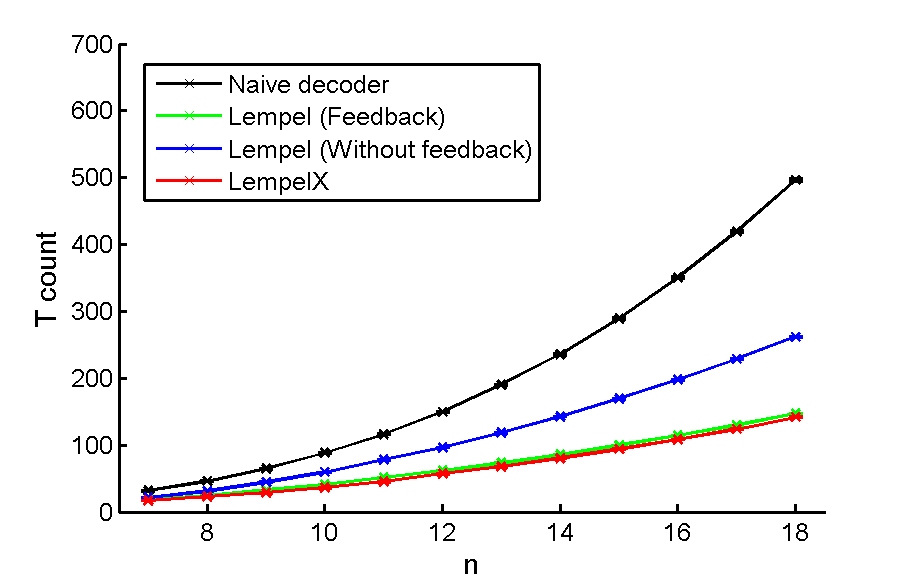
\includegraphics[width=\textwidth]{LX_vs_Lempel}
						\caption{}
					\end{subfigure}
					\begin{subfigure}[b]{0.6\textwidth}
						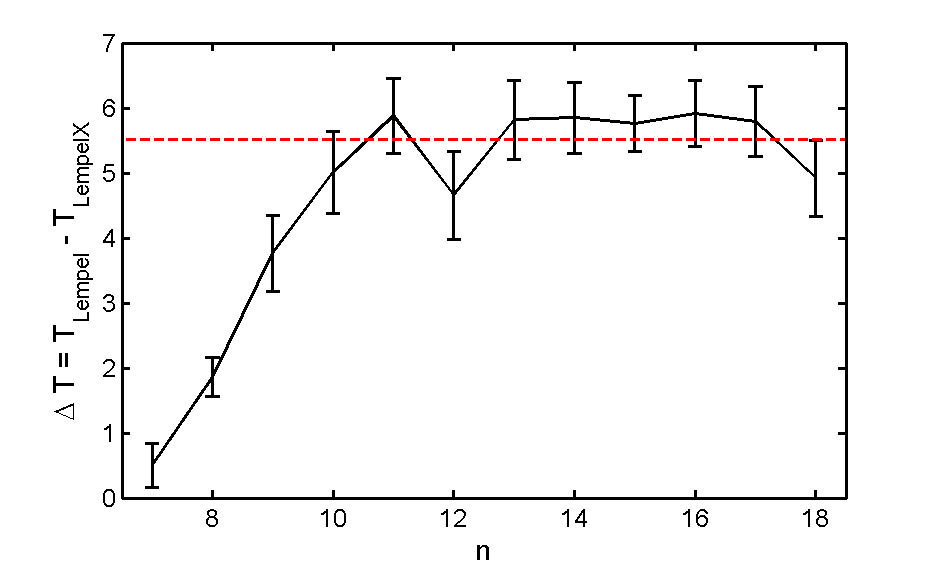
\includegraphics[width=\textwidth]{DeltaT}
						\caption{}
					\end{subfigure}
					\caption{Random Circuits Composed of CNOT and T Gates}
				\end{figure}
				
				\subsection{Universal Practical Circuits}
				Then tested on universal circuits using the following protocol to generalize Toffoli and eliminate Hadamards.
				% Toffoli-n
				\begin{figure}[h]
					\[
					\Qcircuit @C=1em @R=0.7em {
						& \ctrl{1} & \qw & \push{\rule{4em}{0em}} &  & \ctrl{1} & \qw & \ctrl{1} & \qw\\
						& \ctrl{1} & \qw & = &  & \ctrl{3} & \qw & \ctrl{3} & \qw\\
						& \ctrl{1} & \qw & &   &\qw & \ctrl{1} & \qw & \qw \\
						& \targ \qwx & \qw &  &  &\qw & \targ & \qw  & \qw\\
						&&&&\lstick{\ket{0}} & \targ \qwx & \ctrl{-1} & \targ & \qw
					}
					\]		
					\caption{Circuit showing a method to construct the the $4$-control Toffoli gate with standard Toffoli gates. The generalized $n$-controlled Toffoli can be constructed similarly with additional ancillas.}
				\end{figure}
			
				% Removing Hadamards
				\begin{figure}[h]
					\[
					\Qcircuit @C=1em @R=1em {
						\lstick{\ket{\psi}} & \gate{H} &  \rstick{H\ket{\psi}}\qw & &\push{\rule{2em}{0em}=\rule{2em}{0em}} &  \lstick{\ket{\psi}} & \qw & \ctrl{1} & \qw & \qswap & \qw & \qw & \gate{X} & \rstick{H\ket{\psi}}\qw \\
						& & & & & \lstick{\ket{0}} & \gate{H} & \ctrl{-1} & \qw & \qswap \qwx & \qw & \gate{H} & \meter \cwx
					}
					\]
					\caption{This circuit identity is used to trade the internal Hadamards of a circuit for external Hadamards, along with a Pauli-X correction conditioned on the measurement result of an ancilla.}
				\end{figure}
			
			\section{Discussion and Conclusions}
			\label{s6_Discussion}
			
			NOTE: One avenue of improvement especially for the universal construction is to combine T count optimization algorithms with H count optimization such as in (reference). This is likely to complement each other as Hadamard gates serve as obstacles to the T count optimization methods discussed in this report. (Perhaps vice versa). Also would reduce the number of ancillas required to compose multiply controlled toffolis.
			
			NOTE: There may be other conditions that allow for the elimination of gate synthesis matrix columns.
			
			NOTE: It is evident from our analysis of the gate synthesis problem in terms of gate synthesis matrix and signature tensors that the problem is equivalent to determining the symmetric tensor rank of symmetric tensors of order 3. There is likely methods in the Literature that may be adapted for these purposes.
			
			
			
			\bibliographystyle{abbrv}
			\bibliography{keylit} % IMPORTANT! Remember to ammend arXiv references that have been published.
\end{document}